We used our approach on the following use cases:

\subsection{\textbf{Regression Comparison}}
    
\subsubsection{Summary}
    A software company is releasing its new version of software with several new features. The performance regressions tests did not find problems and the unitary tests were accepted. Some weeks after the release, the users started to complain about performance issues in one of the features.
    
\subsubsection{Approach}
    Our approach was to run the software several times on the previous and in the current version of the software. Then classified the data using our approach in slow and fast executions. 
    
    \begin{figure}[h]
      \centering
        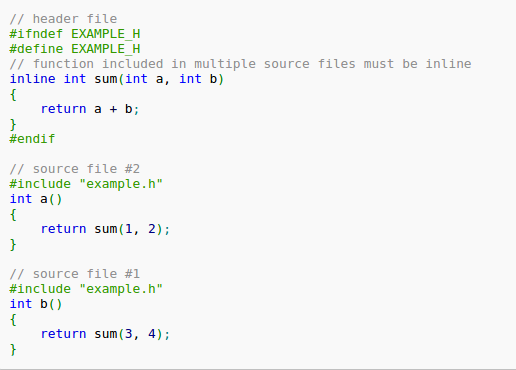
\includegraphics[width=0.50\textwidth]{figures/inline_example.png}
        \caption{Example of Code for inline}
        \label{fig:caseOpt}
    \end{figure}

\subsubsection{Results}
    Were able to find that in-line function addition on the feature increased the number of cache misses and therefore increased the elapsed time of this application. On the source code the in-line functions could be seen as difference although the developers thought that this would improve and not decrease the performance.
    
    Using a comparative approach of the groups we could see the difference of the metrics withing them. Comparing the groups of in-line functions and the groups without inline, we verified that the inline groups comparatively to their respective groups of non-inline, had a significant amount of cache misses. Concluding that cache misses was the essence of the differences.
    
    Table \ref{tab:table}, shows the grouping results relating the cache misses with the slow executions groups comparatively. 
    
\begin{table}[]
\centering
\caption{Table Performance}
\label{tab:table}
\begin{tabular}{ll}
\hline
\multicolumn{2}{c}{Executions}                        \\ \hline
Fast group                & Slow group                \\ \hline
mean of 2500 cache misses & mean of 6500 cache misses
\end{tabular}
\end{table}

\subsection{\textbf{Page Faults Interference}}
    \subsubsection{Summary}
    A program executes several times the process of writing on the buffer, the process reveals a problem after several sub-sequential executions.
    
\subsubsection{Approach}
    Our approach was to run the process several times to trigger this problem. The mechanism classified the executions according to the execution time and also for the metrics.
    
\subsubsection{Results}
     The tree generated had branches with fast and slow executions, 
     The classification was done within the branches of the tree and we were able to find that for all the fast executions (group fast on elapsed time), the group of page-faults were in the first group. On the slow executions, the page-faults were classified on another group. So, the tool revealed the association, and we can conclude that the program triggers more page faults specifically after several executions.\\
     The company was not able to track this problem before because of the prefetching algorithms influence of the executions. This technique is used on the microprocessor architecture to speedup the instructions. The Figure \ref{fig:case1}, is a CCTView result that shows this  difference on the runs on several runs.
    
    \begin{figure}[h]
          \centering
            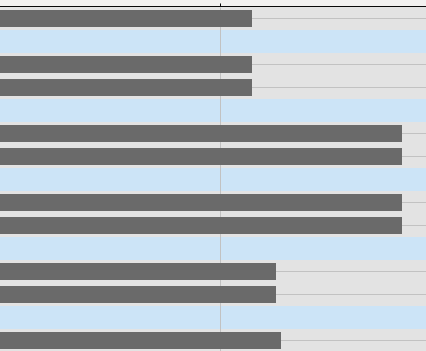
\includegraphics[width=0.50\textwidth]{figures/showing_diff.png}
            \caption{Case study Regression - Tree details showing significantly differences on the runs, where the faster are smaller and the slower are bigger in the images}
            \label{fig:case1}
    \end{figure}
    % Figure \ref{fig:case3}, shows the grouping results relating the page-faults grouping with the slow executions groups.

    
\subsection{\textbf{Cache Optimization in Server Application}}
    
\subsubsection{Summary}
    A server application using a very known content-management framework caches requested data to improve the time access of its content. However, around 1000 requests, the cache is flushed and needs to be redone. So specifically on this request the server will spend more time than on the previous requests.
    
\subsubsection{Approach}
    Our approach was to execute several times a request for a server. While running it, we recorded the tracing data. Then, we executed our clustering analysis and classified the data in several groups.
    
\subsubsection{Results}
    The tree generated by the tool was able to display that on the fast group no time was spent on cache or compile time. However, on slow executions, there was a considerable time spent on compilation time and cache time.
        
    % Figure \ref{fig:case4}, shows the grouping results relating the page-faults grouping with the slow executions groups.
    
    
\subsection{\textbf{Json Cpp}}
\subsubsection{Summary}
    JSON is a lightweight data-interchange format. It can represent numbers, strings, ordered sequences of values, and collections of name/value pairs.

    JsonCpp is a C++ library that allows manipulating JSON values, including serialization and deserialization to and from strings. It can also preserve existing comment in unserialization/serialization steps, making it a convenient format to store user input files.
    
    Executing several times the reading from json file, some of the executions have a different time to read those files.    
    
\subsubsection{Approach}
    Our approach was to run the software several times and run the clustering technique then compared the metrics between the groups.
    The auto-grouping technique showed more than 10 groups to be compared, but only a few were taken in consideration.
    
\subsubsection{Results}
    The solution showed differences on the branches of the tree and was able to display the relation with scheduler switches and the performance of this task, this would impact directly on a real task. All the tasks that took more time were related to task scheduling and switches.
    
    
\subsection{\textbf{OpenCV}}
Open Source Computer Vision Library (OpenCV) is an open source computer vision and machine learning software library. This library is used in different problems in computer vision as tracking image. In this section, we will benchmark Optical Flow and HoughLines algorithms, which they are the most evolving features in the recent years.

\subsubsection{Optical Flow} 
The Optical Flow, implemented as Lucas-Kanade algorithm, is an example of method in OpenCV and aims to correlates the apparent motion of objects between two consecutive frames. From some examples of the book \cite{opencv2_book}, this method can be tested with two images and show differences on them. Regressions can be caused by a series of changes on the code. Doing the tests we found a relevant regression on the function Optical Flow.

\textbf{Approach}: Our approach was to run the software several times recording performance metrics using Linux Perf Events. The elapsed time to track the performance is also used in the classification. The runs were related with several versions of OpenCV until find the regression between the versions 2.3.0 and 2.3.1, where the latest version was around 5 times slower than others.

\textbf{Results}: The results correlate the longer duration with more instructions so we could see on the code that a conditional statement was different from version to another, which makes the slower to execute more instructions. This regression was originally reported on \cite{regression_opencv}.
The total number of commits on those two versions were about 250 commits, using this technique, it was able to reduce the difference for about few lines of code and unit tests can be made to trigger specifically this cause after knowing that it is a cache misses problem.

Figure \ref{fig:OpenCV}, shows the result of the optical flow in from two images.
    
\begin{figure}[h]
      \centering
        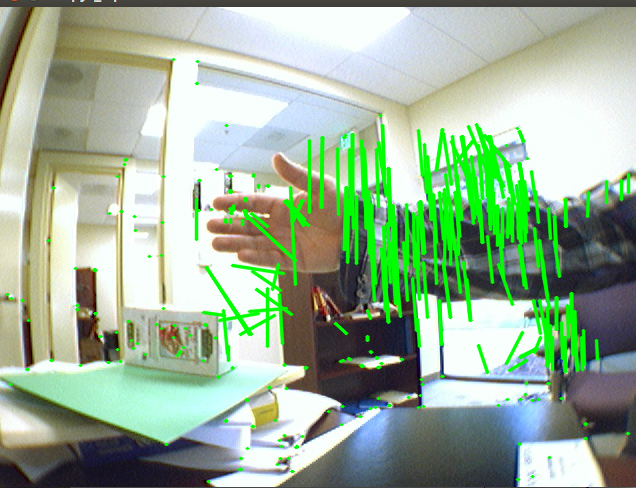
\includegraphics[width=0.50\textwidth]{figures/flow.png}
        \caption{Optical Flow Example}
        \label{fig:OpenCV}
\end{figure}

\subsubsection{HoughLines} 
HoughLines is an line detection mechanism implemented in OpenCV. Comparing different versions, we found that version 3.1 takes more time than version 3.0. in a case of Software Regression. The code difference can be found here \cite{opencv_source_diff}.

\textbf{Approach}: Our approach was to run the software several times recording performance metrics using Linux Perf Events in a large file. The elapsed time to track the performance is also used in the classification. The runs were related with several versions of OpenCV until find the regression between the versions 3.1 and 3.0, where the newer version was slower than the previous one.


\textbf{Results}: The results correlate the longer duration associated the longer runs with cache misses. By analyzing the code we were able to find a difference on the file hough.cpp, related with a difference size of the called array. This process reduced the 
    
    Figure \ref{fig:case2}, shows the grouping results relating the cache misses with the slow executions groups.
    
    \begin{figure}[h]
          \centering
            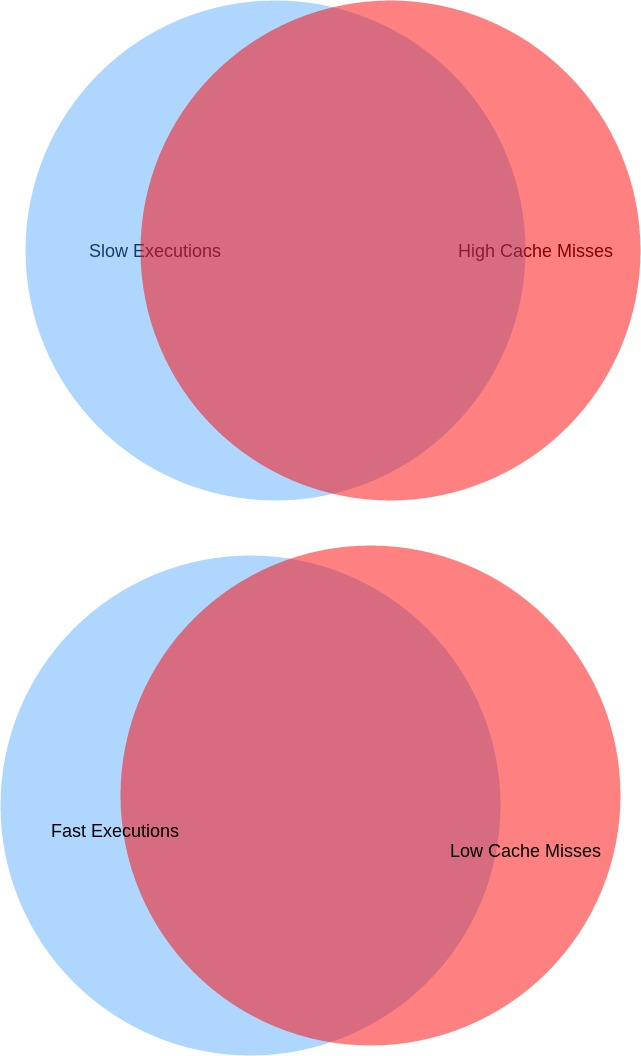
\includegraphics[width=0.350\textwidth]{figures/set_results_cache.jpg}
            \caption{Case study Regression - showing significantly differences in the groups of runs in terms of metrics.}
            \label{fig:case2}
    \end{figure}
    
\subsection{\textbf{Regression Comparison II}}
    
\subsubsection{Summary}
    A software company deployed several new packages in its software including a buffer implementation change. There was a performance impact on this change but it is not possible to track specifically which commit caused the impact. The company would need to run specific Linux commands to find the reason for this problem or reproduce several performance tests with each commit. This scenarios was taken from \cite{essentials} also related to Microsoft bug in \cite{microsoft_bug}.
    
\subsubsection{Approach}
    Our approach was instrument the code and to run the software several times on the previous and in the current version of the software. Then classify the data using our approach in slow and fast executions, although the auto-grouping gave more groups, i.e. reduction of ten to two groups of comparison.
  
\subsubsection{Results}
      The tree generated had branches with fast and slow executions aggregated together. The nodes recorded the several performance metrics including the instructions, cache misses and page-faults.
      We were able to find that page-faults extra addition addition on the feature decreased the performance.
      On the source code, the change on the buffer was an array that was implemented using a row major storage scheme and caused an addition of about 16.384 page faults.
      
      
% \subsubsection{Results}
%      The tree generated had branches with fast and slow executions, 
%      The classification was done within the branches of the tree Figure \ref{fig:case1}, we were able to find that in-line function addition on the feature increased the number of cache misses and therefore increased the elapsed time of this application. On the source code the in-line functions could be seen as difference although the developers thought that this would improve and not decrease the performance.

    The code in highlight shows the difference on the array coding that created the page-faults difference. This code was taken from \cite{essentials}.
    
    % \begin{figure}[h]
    %       \centering
    %         \includegraphics[width=0.2\textwidth]{figures/pf_use_case.png}
    %         \caption{Case study Regression Comparison II - code changes}
    %         \label{fig:caseX}
    % \end{figure}
    

% \begin{lstlisting}
% #include <stdio.h>
% #define N 10
% /* Block
%  * comment */

% int function1()
% {
%     int i;
%     int i, j;
%     int[128][128];
% }
% \end{lstlisting}

\lstset{language=C++,
                basicstyle=\ttfamily,
                keywordstyle=\color{blue}\ttfamily,
                stringstyle=\color{red}\ttfamily,
                commentstyle=\color{green}\ttfamily,
                morecomment=[l][\color{magenta}]{\#}
}
\begin{lstlisting}

    //Considering 128 words/page\\
    
    int i, j;\\
    int[128][128]; \\
    // original version\\
    for(i = 0; i < 128; i++)\\
        for(j = 0; j < 128; j++)\\
            data[i][j] = 0;\\
    // new version\\
    for(j = 0; j < 128; j++)\\
        for(i = 0; i < 128; i++)\\
            data[i][j] = 0;\\

\end{lstlisting}
% \label{pseudo:page-faults}
% 
% \caption{Case  study   Regression  Comparison   II  -  codechanges}
 
